\section{Appendix}

\subsection{Appendix A: Detailed Specification and Design}

\subsubsection{Requirements Specification}

This section restates the requirements introduced in Section~\ref{process} in full, with the source each was elicited from and a MoSCoW priority. Priorities were assigned against the time available: the development environment and the correctness-level author-page defects are treated as \emph{Must}, the interface improvements as \emph{Should}, and the two survey-sourced additions that were ultimately scoped out as \emph{Could}. The status of each requirement and the evidence that verified it are given separately in the traceability table (Table~\ref{tab:traceability}) so that specification and outcome are not conflated.

\begin{table}[h]
\centering
\small
\renewcommand{\arraystretch}{1.2}
\begin{tabular}{@{}l p{0.56\linewidth} l l@{}}
\toprule
\textbf{ID} & \textbf{Requirement} & \textbf{Source} & \textbf{Priority} \\
\midrule
\multicolumn{4}{@{}l}{\textit{Development environment}} \\
\addlinespace[2pt]
DE1 & Run Moodle, CodeRunner and its dependencies in isolation from the host. & Analysis & Must \\
DE2 & Start with a single command and produce a repeatable setup. & Analysis & Must \\
DE3 & Allow CodeRunner to be tested for regressions. & Analysis & Must \\
\addlinespace
\multicolumn{4}{@{}l}{\textit{Functional requirements}} \\
\addlinespace[2pt]
FR1 & Allow the author to delete test cases. & Analysis & Must \\
FR2 & Allow the author to add exactly the number of test cases wanted. & Analysis & Should \\
FR3 & Keep help content visible until the author dismisses it. & Analysis & Could \\
FR4 & Render the Precheck option in its correct column, attached to its test case. & Analysis & Must \\
FR5 & Provide an option to give hints for hidden test cases. & Survey & Could \\
FR6 & Allow the student to save their current work on demand. & Analysis & Should \\
FR7 & Allow the student to manage the layout of the question. & GitHub Issue & Should \\
FR8 & Allow the student to reclaim unused margin space to enlarge the content area. & Analysis & Should \\
FR9 & Provide a copy button on code blocks within the question text. & Survey & Could \\
\addlinespace
\multicolumn{4}{@{}l}{\textit{Non-functional requirements}} \\
\addlinespace[2pt]
NFR1 & Be visually consistent: uniform corner rounding, labels and checkboxes aligned with their controls. & Analysis & Must \\
NFR2 & Score at least 97\% on a Lighthouse accessibility audit. & Analysis & Must \\
NFR3 & Provide documentation that is effective, task-focused and reachable from the question editing form. & Analysis & Must \\
\bottomrule
\end{tabular}
\caption{Requirements specification with elicitation source and MoSCoW priority. Status and verification evidence are in Table~\ref{tab:traceability}.}
\label{tab:requirements-spec}
\end{table}

\subsubsection{System Design}

The system is layered so that the work of this project stays isolated from the platform it extends. At the base is a containerised development environment (Figure~\ref{fig:docker_project}): Docker Compose brings up Moodle on a web-server container, a PostgreSQL database, a JobeInABox sandbox for code execution, a Selenium container for browser tests and a Node container for compiling front-end assets. Moodle and its files live in a managed volume, while the two plugins developed here, the CodeRunner question type and its adapted behaviour dependency, are bind-mounted into that volume from the repository. This arrangement satisfies DE1 and DE2 and means every change is exercised against a real Moodle rather than a mock.

The documentation subsystem was designed for simplicity of authorship and for testability. Content is plain Markdown files under \texttt{docs/editor/}, discovered recursively at request time, so publishing a page requires only adding a file. Rendering is a short pipeline: the raw Markdown is first scanned for an example-list placeholder, which is expanded into per-example import links; it is then transformed to HTML by Moodle's bundled MarkdownExtra parser, configured with a custom \texttt{header\_id\_func} that slugifies each heading into a stable anchor; finally the flat HTML is post-processed to wrap each heading and the content beneath it, up to the next heading, in an anchored \texttt{doc-section} container. Wrapping at this last stage, after transformation, avoids interfering with MarkdownExtra's own block handling. These stages were deliberately extracted from the request script into a library, \texttt{lib/docslib.php}, so that each is a pure function unit-testable in isolation. The page is reachable directly from the question editing form: a documentation link is injected by \texttt{edit\_coderunner\_form.php} above the form body, pointing at the index page, which satisfies the reachability half of NFR3.

The in-plugin search is built on the same section structure. A separate endpoint, \texttt{docs\_searchindex.php}, walks every page and emits a JSON index of sections, each carrying its page, anchor, heading and plain text. The client module, loaded lazily only when the search is first used, fetches this index once and filters it entirely in the browser, which is ample for the small corpus. Ranking favours a whole-phrase match in a heading over one in body text over loose per-word hits, and each result is shown with a breadcrumb of its heading path and a highlighted snippet. The interface is a command palette: a docked bar that opens into a centred modal over a dimmed backdrop, portalled to the document body so that its fixed positioning is measured against the viewport rather than any transformed page wrapper.

Client-side preferences follow a minimal-state design. The layout switcher persists its chosen layout in the browser's \texttt{sessionStorage}, keyed by question id, so a choice survives navigation within a session without being written to the server or tied to the user's identity. No personal data is introduced by any of these changes, and code execution remains isolated on the Jobe sandbox.

\subsection{Appendix B: Detailed Test Strategy and Test Cases}

Testing followed a two-layer strategy. Fast, deterministic PHPUnit tests cover the code this project authored, and the plugin's own browser-driven Behat suite is run unaltered as a regression check on the code the project changed. The extraction of the documentation helpers into \texttt{lib/docslib.php} was undertaken partly to make them unit-testable in isolation, so that the pure logic could be asserted directly rather than only through a rendered page. Security-sensitive input handling is attacked rather than merely exercised: the path-traversal test targets \texttt{../../version.php}, a real file outside the documentation tree, so it cannot be satisfied by a naive existence check. In total the project contributes twenty-seven PHPUnit tests across four files and three Behat scenarios of its own. Every test written for this project passes.

\begin{table}[h]
\centering
\small
\begin{tabular}{@{}p{0.82\linewidth} l@{}}
\toprule
\textbf{Property verified} & \textbf{Result} \\
\midrule
Heading slugification handles spaces, punctuation, casing and empty input & Pass \\
The configured parser is MarkdownExtra and emits \texttt{id} attributes on headings & Pass \\
The documentation directory resolves correctly and contains the index page & Pass \\
Page discovery strips the \texttt{.md} suffix, lists known pages and returns them sorted & Pass \\
Markdown transforms to HTML with anchored headings & Pass \\
Each heading and its body are wrapped in an anchored \texttt{doc-section} container & Pass \\
Content before the first heading is left outside any section & Pass \\
The example-list placeholder expands into per-example import links & Pass \\
Search-index entries carry the page, anchor, heading and text fields & Pass \\
\bottomrule
\end{tabular}
\caption{Unit tests for the documentation library (\texttt{docslib\_test.php}, 9 tests).}
\label{tab:tests-docslib}
\end{table}

\begin{table}[h]
\centering
\small
\begin{tabular}{@{}p{0.82\linewidth} l@{}}
\toprule
\textbf{Property verified} & \textbf{Result} \\
\midrule
A valid page renders inside the normal Moodle page chrome & Pass \\
An absent page parameter defaults to the index page & Pass \\
An XML sample is streamed verbatim as a download & Pass \\
The examples page expands the example list with per-example import links & Pass \\
The walkthroughs page renders with its import links & Pass \\
A path-traversal request (\texttt{../../version.php}) raises a Moodle exception & Pass \\
A request for a nonexistent page raises a Moodle exception & Pass \\
\bottomrule
\end{tabular}
\caption{Integration tests for the documentation page (\texttt{docs\_page\_test.php}, 7 tests).}
\label{tab:tests-docspage}
\end{table}

\begin{table}[h]
\centering
\small
\begin{tabular}{@{}p{0.82\linewidth} l@{}}
\toprule
\textbf{Property verified} & \textbf{Result} \\
\midrule
The course chooser lists only courses the user may edit & Pass \\
The chooser warns when no editable course is available & Pass \\
An import creates the questions inside an examples category & Pass \\
An import is denied without the required capability & Pass \\
An import is denied without a valid session key & Pass \\
An invalid example slug is rejected & Pass \\
A repeated import reuses the single existing examples category & Pass \\
A failing import reports the failure and imports nothing & Pass \\
An import is refused on an incompatible \texttt{mod\_qbank} site & Pass \\
\bottomrule
\end{tabular}
\caption{Tests for the one-click example importer (\texttt{import\_example\_test.php}, 9 tests).}
\label{tab:tests-import}
\end{table}

\begin{table}[h]
\centering
\small
\begin{tabular}{@{}p{0.82\linewidth} l@{}}
\toprule
\textbf{Property verified} & \textbf{Result} \\
\midrule
Deleting a test case from the middle of the form keeps the survivors correctly paired & Pass \\
Validation maps each surviving test case back to its original form row number & Pass \\
\bottomrule
\end{tabular}
\caption{Tests for the test-case indexing rewrite (\texttt{questiontype\_test.php}, 2 tests added by this project).}
\label{tab:tests-questiontype}
\end{table}

For acceptance testing the unmodified upstream Behat suite is executed against the Selenium container, providing independent regression evidence for the test-case indexing rewrite (DE3). Three Behat scenarios were additionally written for the project's own features: \texttt{layoutswitcher.feature} (FR7 and FR8), \texttt{docs\_navigation.feature} (NFR3) and \texttt{authorform\_docs\_link.feature}, which confirms the documentation link on the editing form is present and opens the index page. All three pass.

\paragraph{Commentary on results.} The results are uniformly green because the suites were kept small and deterministic and each was run to completion before being recorded; their value therefore lies less in the pass rate than in what the tests attack. The documentation tests are weighted towards the two places that can genuinely fail: the path-containment defence, probed with a real out-of-tree file rather than a fabricated one, and the section-wrapping and search-index logic on which the in-plugin search depends. The two question-type tests target a specific, previously latent defect: before the indexing rewrite, deleting a test case from the middle of the form silently dropped a survivor, and these tests fail against the original contiguous-index code, so they document the regression as much as they guard against it. The importer tests deliberately include the unhappy paths, denied capability, missing session key, bad slug, duplicate category and outright import failure, because those are the paths a one-click action is most likely to get wrong. The honest limit is the shape of the coverage rather than its depth: the interactive JavaScript features are reached only by the three project Behat scenarios and by manual review, and the upstream Behat suite, while a strong regression signal, is occasionally flaky at the browser layer and is treated as such rather than as a precise measure.

\subsection{Appendix C: User Guide}

The full user guide, covering how to run the system and how to use the author- and student-facing features the project delivers, is provided online rather than inline to conserve space. It is hosted alongside the project's deployed instance at \url{https://moodle.skraburski.com}, and fuller setup notes, including prerequisites and host configuration, remain in the repository's \texttt{README}.

\subsection{Appendix D: Ethics Documentation}

Due to page-count limitations, online-only versions of the \emph{participant information sheet} and \emph{consent form} can be found at the links below. Each respective section contains the same file; multiple hosts were used to provide backup sources. 
\subsubsection{Ethical Approval Form}
\begin{figure}[h]
    \centering
    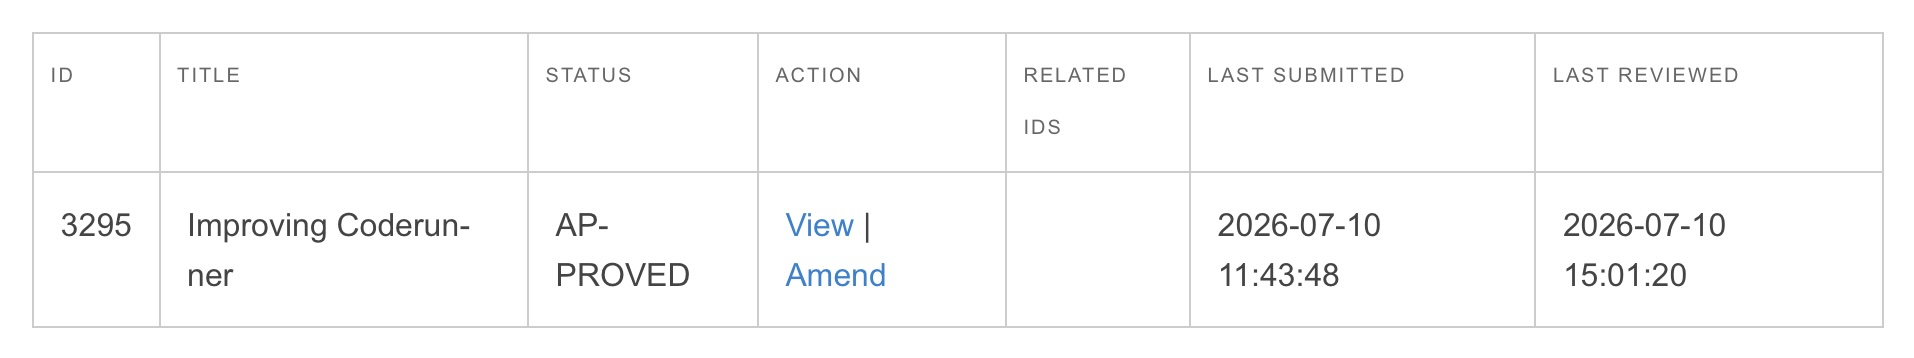
\includegraphics[width=0.7\textwidth]{figs/approval.jpg}
    \caption{Ethical Approval found on the Strathclyde Ethics page}
    \label{fig:ethicsapproval}
\end{figure}

\subsubsection{Participant Information Sheet}
\emph{Github:} \url{https://github.com/michal-skraburski/mono-moodle-docker/blob/main/survey/information/Participant%20Information%20Sheet%20for%20Survey%20of%20Improving%20Coderunner.pdf}


\emph{Microsoft Sharepoint:} \url{https://strath-my.sharepoint.com/:b:/g/personal/michael_skraburski_2022_uni_strath_ac_uk/IQCZ9rzUDisVQ5cogEBKp8NaAZVEz6FbEr3ZcyZ0uesNYtE?e=LWoPEE}
\subsubsection{Consent Form}
\emph{Github:} \url{https://github.com/michal-skraburski/mono-moodle-docker/blob/main/survey/information/consent%20form%20Coderunner.pdf}


\emph{Microsoft Sharepoint:} \url{https://strath-my.sharepoint.com/:b:/g/personal/michael_skraburski_2022_uni_strath_ac_uk/IQBuEWi08Wb9SIbs33qZy9SsASCw3drzVzA__IZTQId0BH0?e=Hem5ae}
